\section{Refactorización de FuD}

\begin{frame}{Refactorización de FuD}
%     \begin{block}{}\centering \rc{} $+$ \fud{} $\neq$ articulación 100\%\end{block}

        \centering
        \only<1-3>{
\includegraphics[scale=0.4]{images/fud-recabs-non-compatible.png}}
%             \centering
        \only<4>{
\includegraphics[scale=0.4]{images/fud-recabs-compatible.png}}

    \vspace{0.5cm}
    \pause
    \begin{center}
        \begin{Large}¿Qué faltaba en \fud{}?\end{Large}
        \vspace{0.7cm}
        \pause
        \begin{itemize}
            \item  Envío de mensajes de cliente a servidor.\\ \rc: \textit{envío de resultados y trabajos en cualquier momento}.
            \vspace{0.2cm}
            \pause
            \item  Pedido y reserva de clientes.\\ \rc: \textit{balanceo de carga dinámico con respecto a disponibilidad de clientes}.
        \end{itemize}

    \end{center}

\end{frame}


\subsection{Diseño}

\begin{frame}{Diagrama de clases}
    \only<1>{
        \centering
            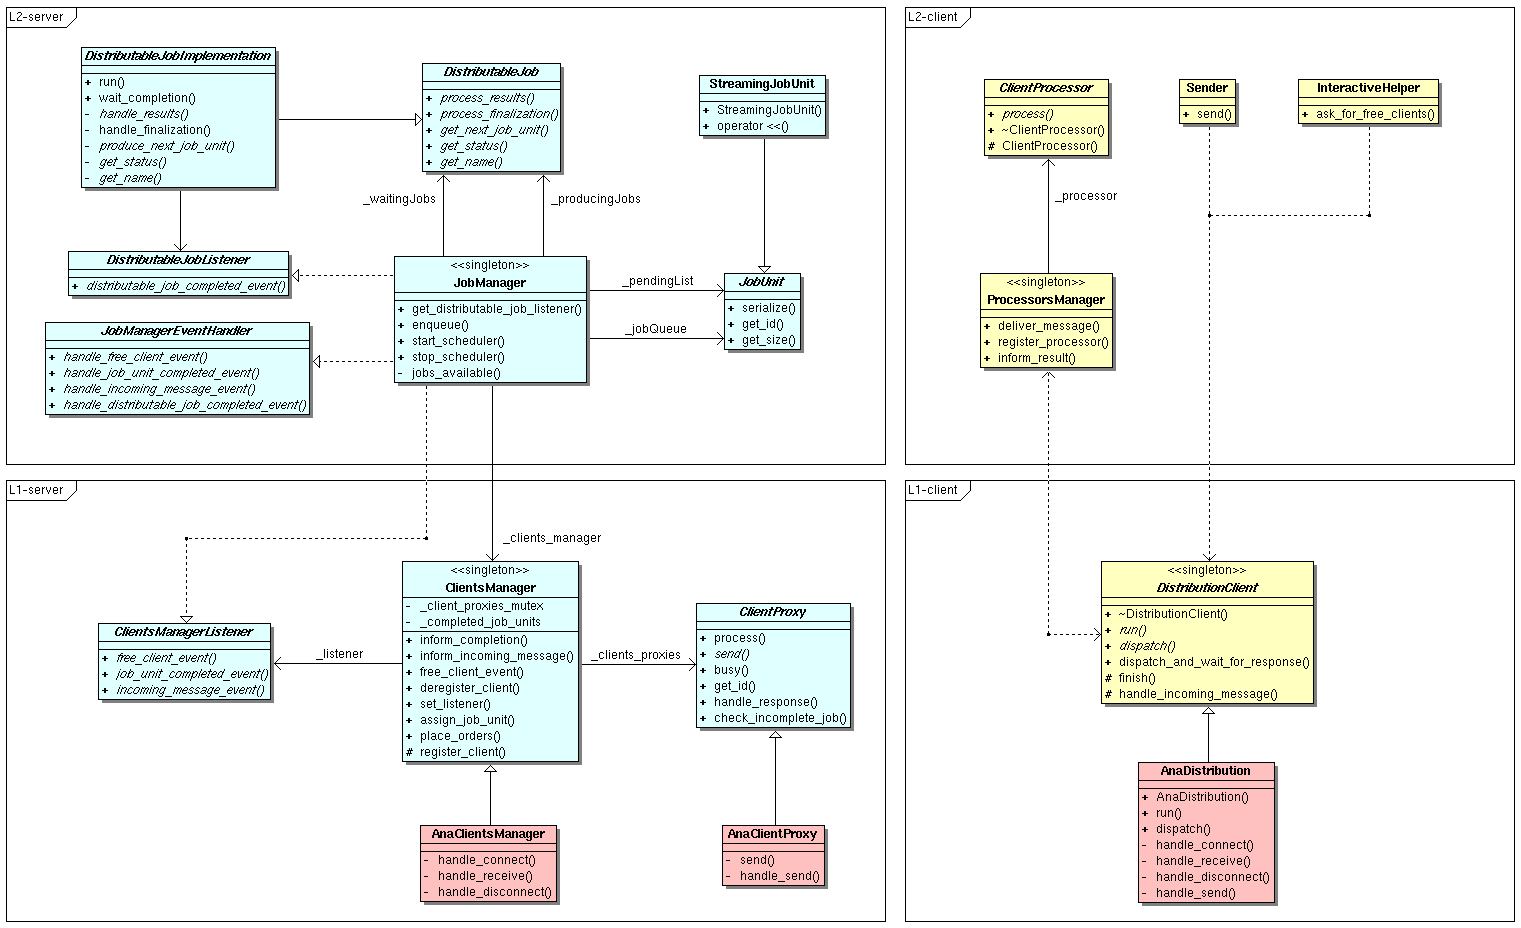
\includegraphics[scale=0.21]{images/fud_class.png}
    }
    
    \only<2>{
        \begin{center}
            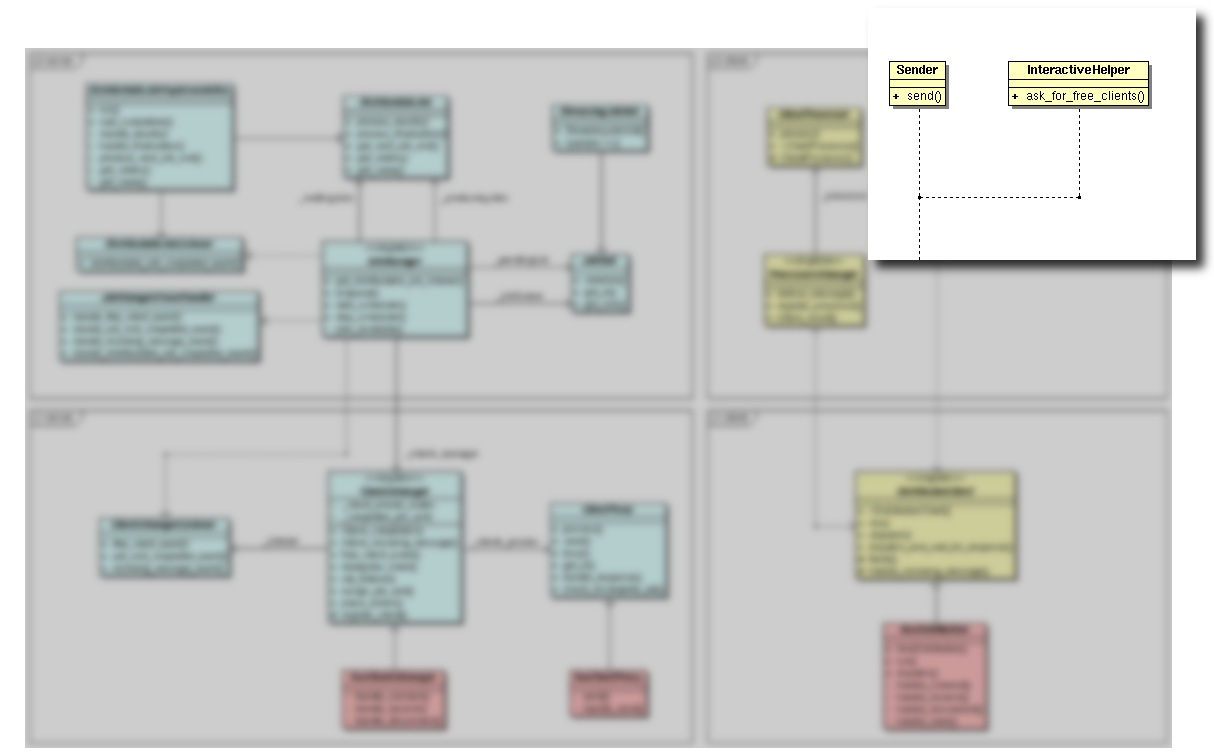
\includegraphics[scale=0.21]{images/fud_class-zoom.png}
        \end{center}
    }

\end{frame}

\begin{frame}{Lado Cliente: Antes}
    \begin{columns}[T]
        \begin{column}{.6\textwidth}
            \centering
            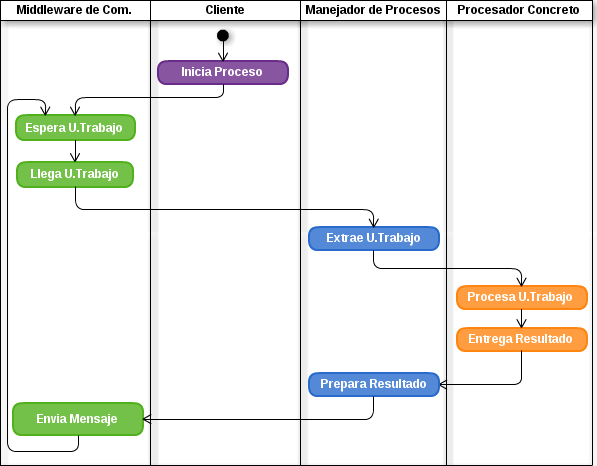
\includegraphics[scale=0.3]{images/ActivityFuDClient-Orig.png}
        \end{column}
        \begin{column}{.4\textwidth}
            \begin{enumerate}
                \item   Cliente recibe trabajo y lo procesa.
                \vspace{0.2cm}
                \item   Finalización del trabajo con envío de resultado final.
            \end{enumerate}
        \end{column}
    \end{columns}
\end{frame}

\begin{frame}{Lado Cliente: Después}
    \begin{columns}[T]
        \begin{column}{.6\textwidth}
            \centering
            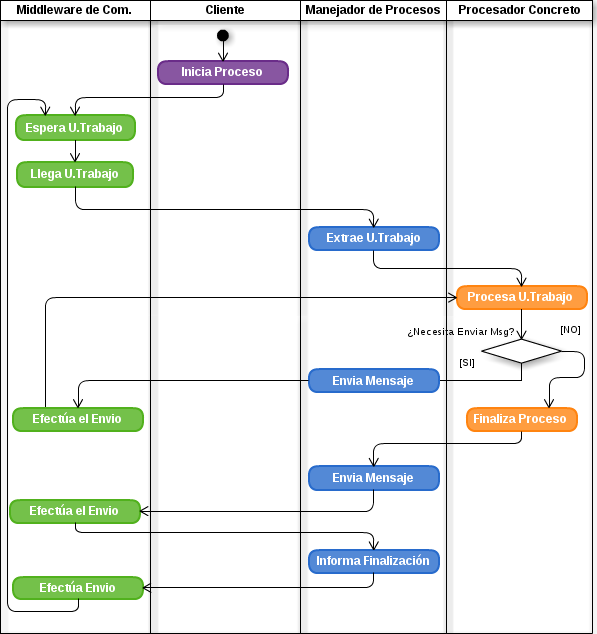
\includegraphics[scale=0.3]{images/ActivityFuDClient-Duplex.png}
        \end{column}
        \begin{column}{.4\textwidth}
            \begin{enumerate}
                \item   Cliente recibe trabajo, y empieza a procesar.
                \vspace{0.2cm}
                \item   Opción de enviar mensajes y/o trabajos no procesados.
                \vspace{0.2cm}
                \item   Finalización.
            \end{enumerate}
        \end{column}
    \end{columns}
\end{frame}

\begin{frame}{Lado Servidor: Antes}
    \begin{columns}[T]
        \begin{column}{.55\textwidth}
            \centering
            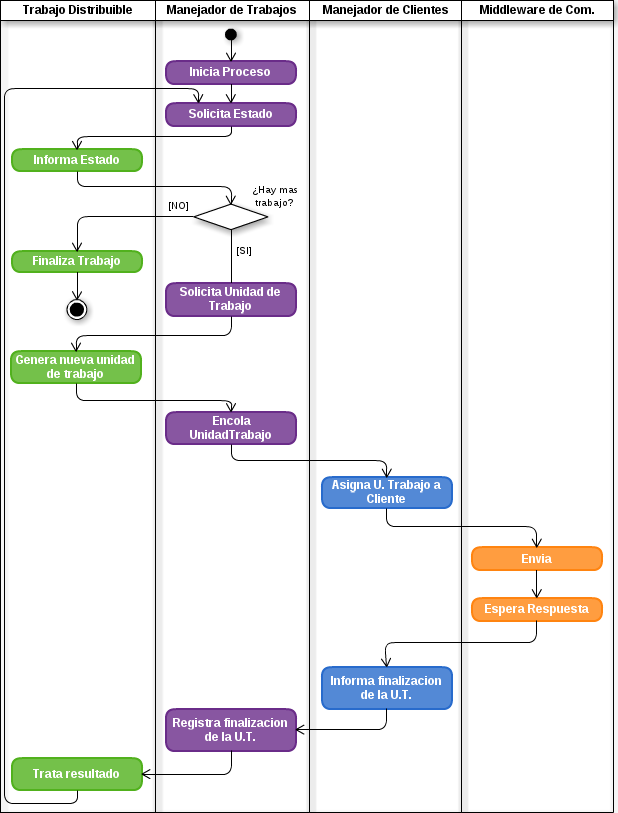
\includegraphics[scale=0.23]{images/ActivityFuDServer-Orig.png}
        \end{column}
        \begin{column}{.45\textwidth}
            \begin{enumerate}
                \item   Verifica si hay trabajos pendientes
                \vspace{0.2cm}
                \item   Genera unidad de trabajo (U.T.)
                \vspace{0.2cm}
                \item   Asigna U.T. a cliente libre
                \vspace{0.2cm}
                \item   Espera resultado final
                \vspace{0.2cm}
                \item   Finalización de U.T.
            \end{enumerate}
        \end{column}
    \end{columns}
\end{frame}

\begin{frame}{Lado Servidor: Después}
    \begin{columns}[T]
        \begin{column}{.55\textwidth}
            \centering
            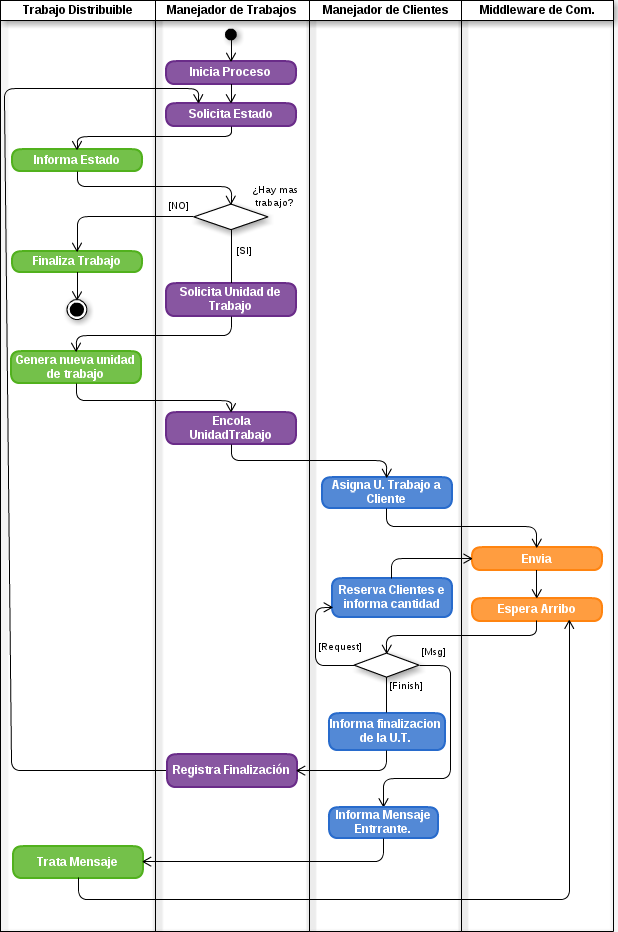
\includegraphics[scale=0.2]{images/ActivityFuDServer-Duplex.png}
        \end{column}
        \begin{column}{.45\textwidth}
            \begin{enumerate}
                \item   Verifica si hay trabajos pendientes
                \vspace{0.2cm}
                \item   Genera unidad de trabajo (U.T.)
                \vspace{0.2cm}
                \item   Asigna U.T. a cliente libre
                \vspace{0.2cm}
                \item   Espera mensaje, requerimiento de clientes libres o finalización de U.T.
                \vspace{0.2cm}
                \item   Trata mensaje correspondiente
                \vspace{0.2cm}
                \item   Finalización de U.T.
            \end{enumerate}
        \end{column}
    \end{columns}
\end{frame}


\subsection{Implementación}

\begin{frame}{Dependencias}
    La refactorización de \fud{} incluyó las siguientes librerías:
    \begin{description}
        \item[MiLi]: colección sencilla de pequeñas librerías útiles.
        \item[ANA]: librería de red asincrónica.
    \end{description}
\end{frame}

\begin{frame}{Métricas}
    La refactorización de \fud{} implicó la modificación de 21 archivos y la creación de 5 archivos, con un total de 1114 líneas de texto.
    \begin{center}
        \rowcolors{2}{verde!20}{verde!5}
        \begin{tabular}{|l|r|r|r|r|r|c|}
            \hline
            \multicolumn{3}{|c|}{Files} & \multicolumn{3}{|c|}{Line Types} & \hspace{0.2cm}\% \\
            \hline
            \textbf{Type} & \textbf{Mod.} & \textbf{Cre.} & \textbf{Blank} & \textbf{Com.} & \textbf{Source} & \small{\textbf{Com./Tot.}}\\
            \hline
            \texttt{C++ source} & 9   & 3   &    60  &    176   &   287 & 38.01 \\
            \hline
            \texttt{C++ header} & 12  & 2   &    88  &    403   &   100 & 80.11 \\
            \hline
            \textbf{Total}      & 21  & 5   &   148  & \color{blue}579\color{black} & \color{blue}387\color{black} & \textbf{59.93} \\
            \hline
        \end{tabular}
    \end{center}
\end{frame}